\indent
Рассмотрим поведение конденсатора при постепенном увеличении частоты. Пусть сначала к обкладкам конденсатора приложено переменное напряжение низкой частоты. Когда напряжение меняется, с нижней обкладки положительный заряд сменяется отрицательным. Заряд медленно "плещется" туда-сюда и поле вместе с ним. В каждый момент времени электрическое поле однородно (без учета краевых эффектов). Электрическое поле в этом случае можно записать в виде
\begin{equation}
    E = E_0 e^{i\omega t},
\end{equation}
где $E_0$ постоянно. \\
\indent
Однако, при изменениии электрического поля, согласно уравнениям Максвелла, возникает магнитное поле.
\begin{equation}
    \oint_L \mathbf{H}d\mathbf{l} = \frac{4\pi}{c}\int_S \left(\mathbf{j} + \frac{1}{4\pi}\frac{\partial \mathbf{D}}{\partial t}\right)d\mathbf{S} \label{eq:max_1}
\end{equation}
В силу симметрии магниное поле будет направлено по концентрическим окружнжостям вокруг электрического поля. Тогда при условии отсутсвия токов проводимости ($\mathbf{j} = 0$) и для простоты вычислений $\varepsilon = \mu = 1$
$$ B \cdot 2\pi r = \frac{1}{c}\frac{\partial E}{\partial t} \cdot \pi r^2\\ $$

Получаем выражение магнитной индукции в зависимости от радиуса $r$
\begin{equation}
    B = \frac{i\omega r}{2 c}E_0 e^{i\omega t}\label{eq:B1}
\end{equation}
Видим, что магнитное поле тоже колеблется, ес
SOMETHING!!!! page 202

\indent
Теперь будем увеличивать частоту и посмотрим, что происходит. Т.к магнитное поле тоже изменяется со временем, то электрическое поле уже не может считаться однородным. Согласно уравнениям Максвелла должна возникнуть вихревое электрическое поле, которое будет изменятся в зависимости от $r$:
\begin{equation}
    \oint_L \mathbf{E}d\mathbf{l} = -\frac{1}{c}\int_S \frac{\partial \mathbf{B}}{\partial t}d\mathbf{S} \label{eq:max_2}
\end{equation}

\indent
Пусть электрическое поле при низких частотах $\mathbf{E_1} = \mathbf{E_0} e^{i\omega t}$ и $\mathbf{E_2}$ - поправка из-за изменения магнитного поля. Тогда суммарное поле:
$$ \mathbf{E} = \mathbf{E_1} + \mathbf{E_2}$$
В центре конденсатора при $r = 0$ будем считать $E_2 = 0$.\\
\indent
Чтобы найти $E_2$ используем выражение \ref{eq:max_2}.

\newpage
\begin{figure}[h!]
    \centering
    \begin{subfigure}{0.48\linewidth}
        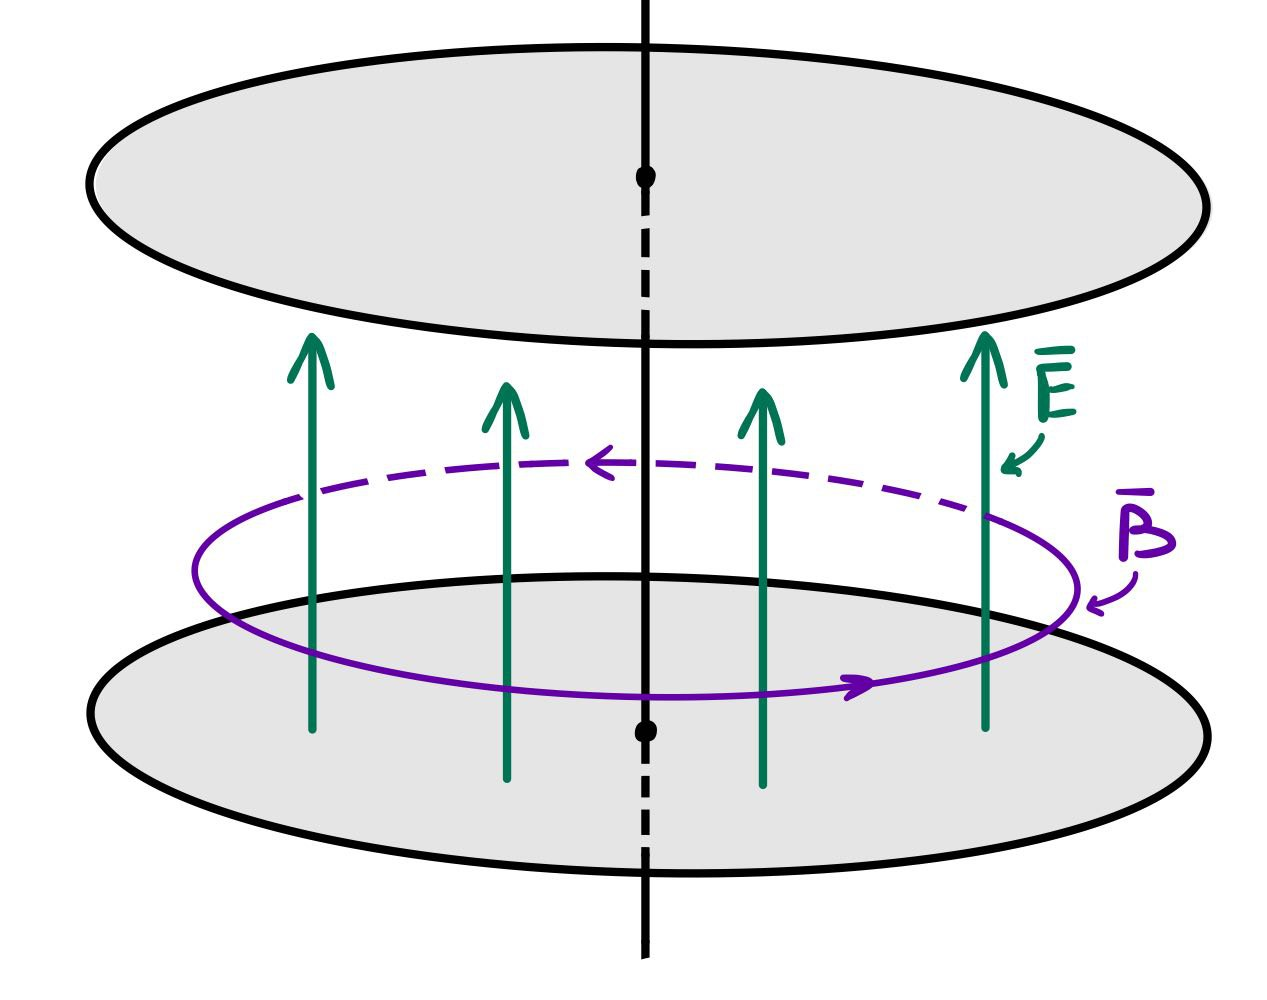
\includegraphics[width = 8cm]{images/cond1.jpg}
    \end{subfigure}
    \begin{subfigure}{0.48\linewidth}
        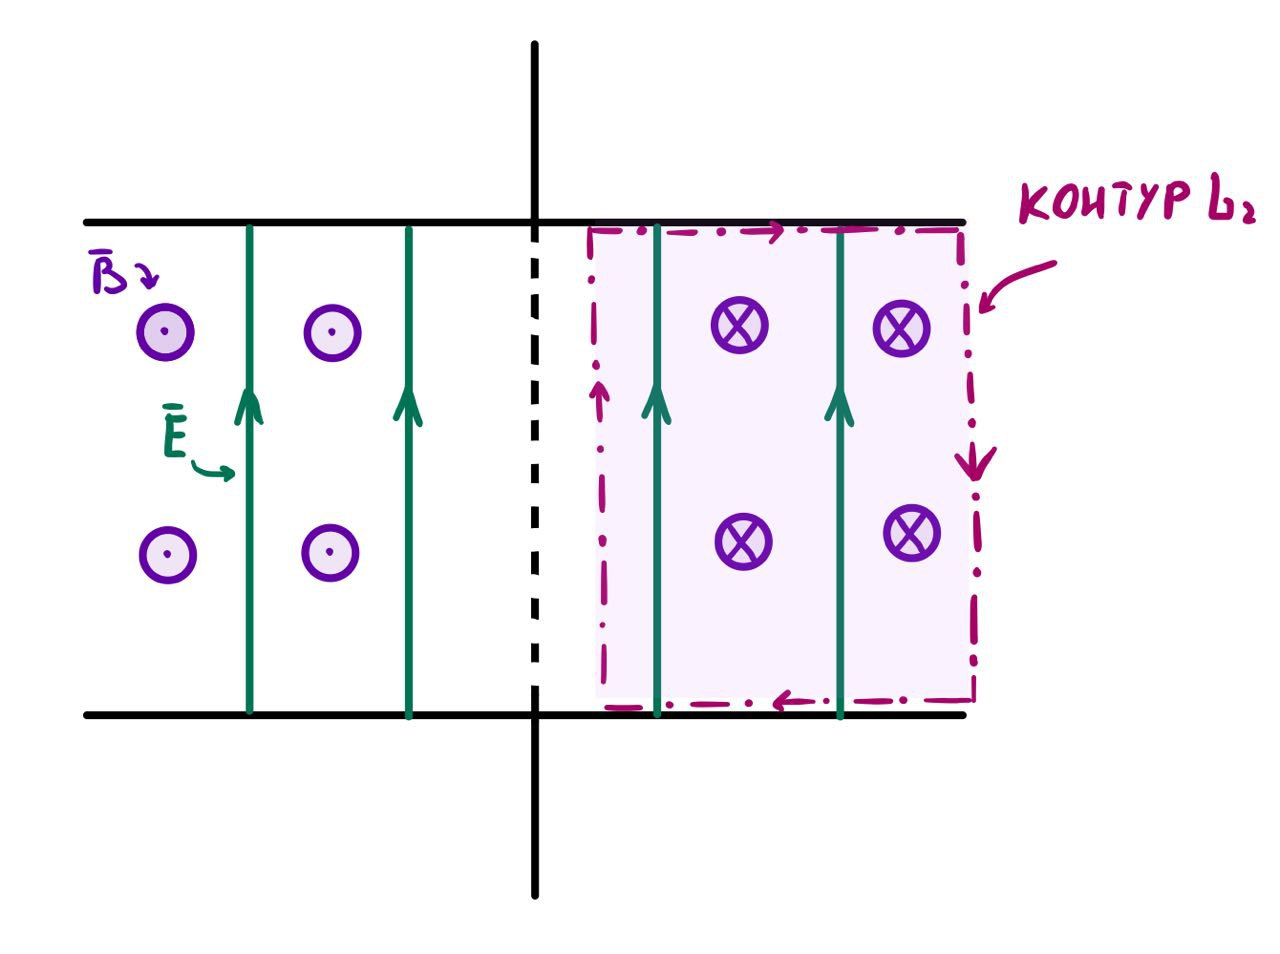
\includegraphics[width = 8cm]{images/cond2.jpg}
    \end{subfigure}
    \caption{Электрическое и магнитное поля между обкладками конденсатора} \label{table:cond}
\end{figure}

\noindent
Цикруляцию электрического поля берем по контуру $L_2$, изображенному на \ref{table:cond}. Получаем 
$$-E_2(r) \cdot h = -\frac{1}{c}\int_{0}^{r} \frac{\partial B}{\partial t} \cdot h dr,$$
где $h$ - расстояние между обкладками конденсатора.
\begin{equation}
    \mathbf{E_2} = -\frac{\omega^2 r^2}{4 c^2}\mathbf{E_0} e^{i\omega t}
\end{equation}
\begin{equation}
    \mathbf{E} = \left (1 - \frac{1}{4}\frac{\omega^2 r^2}{c^2}\right ) \mathbf{E_0} e^{i\omega t}
\end{equation}

\begin{wrapfigure}{r}{0.48\linewidth}
    \centering
    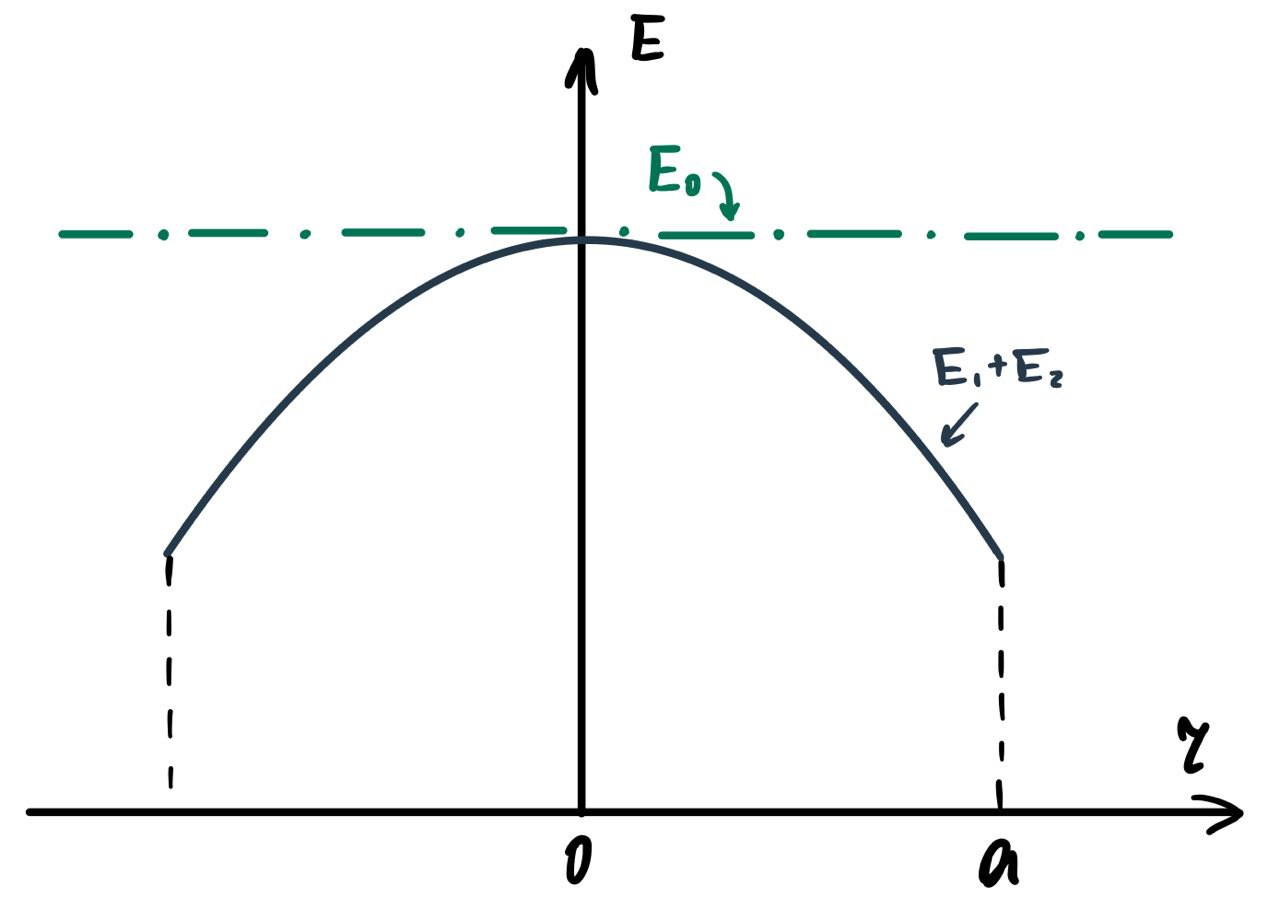
\includegraphics[width=8cm]{images/plot1.jpg}
    \caption{Электрическое поле между обкладками конденсатора на высоких частотах}
\end{wrapfigure}

\indent
Может показаться, что на этом наши рассуждения подошли к концу, однако выражение для поля $B$ \ref{eq:B1} верно только в первом приближении. Перепишем его как 
$$B_1 = \frac{1}{2}\frac{i\omega r}{c} E_0 e^{i\omega t}$$
Т.к это поля появилось из-за изменения $\mathbf{E_1}$, а правильное магнитное поле будет создаваться от электрического поля $\mathbf{E_1} + \mathbf{E_2}$. Аналогично тому, как мы поступали с электрическим полем, представим магнитное в виде $\mathbf{B} = \mathbf{B_1} + \mathbf{B_2}$, где $\mathbf{B_2}$ - добавочное поле, создаваемое полем $\mathbf{E_2}$. Снова применим теорему о цикруляции магниной индукции \ref{eq:max_1}:
$$B_2 \cdot 2 \pi r = \frac{1}{c} \int_{0}^{r} \frac{\partial E_2(r)}{\partial t} \cdot 2\pi rdr$$

Получаем выражение для $B_2$:
\begin{equation}
    B_2(r) = -\frac{1}{16}\frac{i\omega^3 r^3}{c^3}E_0 e^{i\omega t}
\end{equation}

\indent
Но раз магнитное поле снова не такое, как мы изначально думали, то надо посчитать еще одну поправку к $\mathbf{E}$\dots Однако новое электрическое поле вызовет новую поправку к магнитному полю, которое в свою очередь приведет к дальнейшей поправке к электрическому полю и т.д и т.д.

\indent
Таким образом, выражение для напряженности электрического поля можно записать как:
\begin{equation}
E = E_0 e ^{i\omega t}\left(1 - \frac{1}{(1!)^2}\left(\frac{\omega r}{2 c}\right)^2 + \frac{1}{(2!)^2}\left(\frac{\omega r}{2 c}\right)^4 - \frac{1}{(3!)^2}\left(\frac{\omega r}{2 c}\right)^6 + \dots \right)
\end{equation}
И выражение для индукции магнитного поля:
\begin{equation}
    B = E_0 e^{i\omega t}\left (
        \frac{1}{1!}\left (\frac{\omega r}{2 c}\right )^{1} - 
        \frac{1}{1!2!}\left (\frac{\omega r}{2 c}\right )^{3} + 
        \frac{1}{2!3!}\left (\frac{\omega r}{ 2 c}\right )^{5} - 
        \frac{1}{3!4!}\left (\frac{\omega r}{ 2 c}\right )^{7} +  \dots 
    \right )
\end{equation}
\indent
Окончательно получается, что электрическое поле между обкладками конденсатора на любой частоте дается произведением $E_0 e^{i\omega t}$ на бесконечный ряд, содержащий переменную $\omega r / c$. Аналогично и для поля $B$.\\
\indent
Обозначим $x = \frac{\omega r}{c}$. Тогда выражения для $E$ и $B$ примут следующий вид:
\begin{align}
    E &= E_0 e ^{i\omega t}\left(
    1 - \frac{x^2}{(1!)^2}+ 
    \frac{x^4}{(2!)^2} - 
    \frac{x^6}{(3!)^2} + \dots 
\right) = \sqrt{\frac{2}{\pi x}}\cos \left (x - \frac{\pi}{4} \right )\\
B &= E_0 e^{i\omega t}\left (
        \frac{x}{1!} - 
        \frac{x^3}{1!2!}+ 
        \frac{x^5}{2!3!} + \dots 
    \right ) = \sqrt{\frac{2}{\pi x}}\cos \left (x - \frac{3\pi}{4} \right )
\end{align}
Последнее равентсво верно для $x \ll 1$. Эти функции называют функциями Бесселя 1-го рода 0-го $J_0(x)$ и 1-го $J_1(x)$ порядка соответсвтенно.
\begin{figure}[h!]
    \centering
    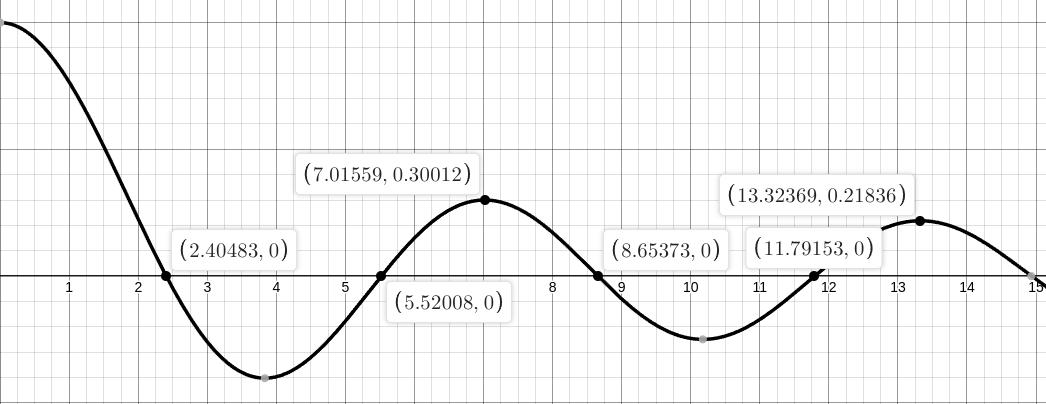
\includegraphics[width=14cm]{images/bessel_j0.png}
    \caption{Функция Бесселя $J_0(x)$}
\end{figure}
\begin{figure}[h!]
    \centering
    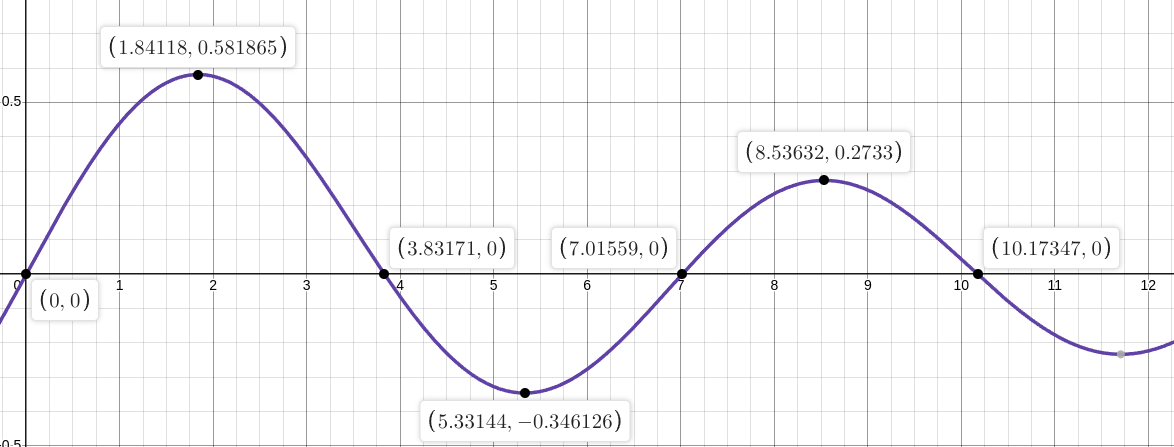
\includegraphics[width=14cm]{images/bessel_j1.png}
    \caption{Функция Бесселя $J_1(x)$}
\end{figure}
\newpage

\indent
Из графиков видно, что поля в центре конденсатора и у его края могут быть направлены в противоположные стороны. И вообще по мере удаления от центра конденсатор может много раз менять направление своих полей. При высоких частотах конденсатор уже не напоминает идеальной емкости. Конденсатор похож, с одной стороны, на емкость, а с другой - на индуктивность. От электрического поля возникают заряды на поверхности обкладок, а от магнитного - ЭДС.

